\section{Environment}

%This section describes the developed task environment for answering the research question. First of all a brief explanation will be given of what the task environment is. 
%Then in the first section the components of the environment are described followed by a discussion of the different manipulation tasks and the Leap Motion and keyboard and mouse 
%control interfaces.

The task environment is a virtual graphical computer program for building virtual block structures using either a Leap Motion or keyboard and mouse. It was developed in order 
to answer the research question and was created with the use of jMonkeyEngine~\cite{Irene:2012}~\footnote{More on jMonkeyEngine: \url{http://jmonkeyengine.org/}}, an open source 
3D game engine written in Java. The Software Development Kit that came with the engine provided a high level interface for numerous 3D functions and data-structures (e.g. shaders, 
spatial manipulation, quaternions and 3D meshes) and also provided a high degree of control for developers by being completely compatible with the Java programming language. 
Section~\ref{sec:components} describes the components of the environment in detail.

The task environment has been developed for being a general interface were the components can be controlled either with the Leap Motion or with the keyboard and mouse through different 
control interfaces. Switching between the two control interfaces was managed through a simple setting in a configuration file. The Leap Motion control interface was developed through 
the Leap Motion SDK~\footnote{Leap Motion developer: \url{https://developer.leapmotion.com/}}. Both control interfaces are described in more detail in section~\ref{sec:interface}.

% The environment is manipulated with the Leap Motion device or with the mouse control interfaces  that are described in section~\ref{sec:interface}. employ the Leap Motion SDK.

%Therefore most of the components of the environment are utilized by both control strategies.

\subsection{Components}\label{sec:components}

\begin{figure}[H]
\centering
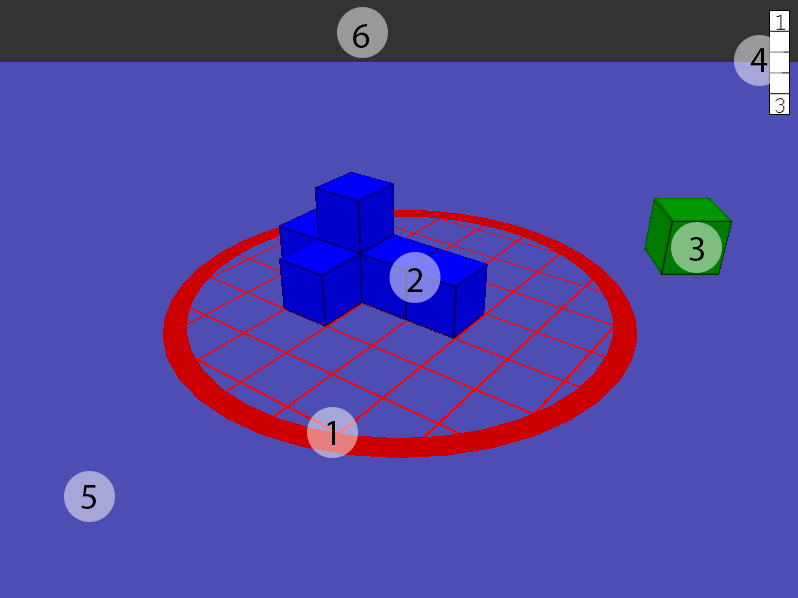
\includegraphics[width=\textwidth]{env_comps}
\caption{\label{fig:environmentcomps} Common rendering of the task environment. Visual elements: 1-Circular~grid 2-Building~blocks 3-Creation~block 4-Target~indicator 5-Floor 
6-Horizon}
\end{figure}

\noindent Figure~\ref{fig:environmentcomps} shows a common rendering of the task environment, seen through the lens of a virtual camera, in which all visual elements have been 
labeled. In the center of the screen users were presented with a circular grid that was segmented into several squares, effectively representing a grid with a circular border. 
On this grid building blocks could be positioned, either directly on the grid or stacked on top of other building blocks. New building blocks could be obtained by interacting 
(clicking with the mouse or grabbing with the Leap Motion) with the creation block just next to the circular grid. The target indicator on the top right corner gave the user a 
representation of the block structure that was supposed to be created on the grid before the user could advance.

\paragraph{Circular grid}
The circular grid was made out of square grid-cells and a limit circle with a radius that was slightly bigger than $3.5$ grid-cells width. The grid was able to rotate 
$360^{\circ}$ around the y-axis of the center of this grid (the origin). In resting state the grid and limit circle had a red color, but while the circle was rotated by the 
user the limit circle temporarily became orange until it reached resting state once more. 

\paragraph{Camera}
The camera component determined what was seen on the screen and had the origin of the circular grid as the focal point. The camera was always positioned at a fixed 
distance of $13 \frac{1}{3}$ grid-cells width from the origin of the circular grid. It started at a position in front of the circular grid under an angle of $45^{\circ}$ relative to the grid origin. The angle of the camera was modifiable in order to change the perspective on the circular grid, but the angle was limited between $1^{\circ}$ and $89^{\circ}$.

\paragraph{Building blocks}
The building blocks were 3D cubes with dimensions corresponding to $1\times 1\times 1$ the width of a grid-cell within the grid and all having black outlines at the edges. Building blocks could be lifted, dragged around, and dropped by the user. While building blocks were lifted they cast a shadow directly below them in order to let the user know their position relative to the floor and other building blocks. When building blocks were lifted and within the radius of the grid, they automatically aligned towards the grid-cells. In resting state the building blocks were blue, when they were being dragged they were orange and when a user pointed at them, but was not dragging any blocks, they became light-blue. When building blocks were released they were subjected to gravity, i.e. they fell until they hit the floor or another building block. If building blocks were released outside the circular grid they dissolved and were discarded.

\paragraph{Creation block}
The creation block was an unique fixed-position building block with the same dimensions as a building block, but with a different color. A user could use the creation block to obtain new building blocks by interacting with it. When a user pointed at the creation block it turned light-green, otherwise it had a dark-green color. In the version of the environment used for the experiment the creation block was positioned one grid-cell width above the floor level to compensate for the limited vertical detection range of the Leap Motion. Also depending on the handiness of the user the creation block was either positioned on the left (for left-handed users) or positioned on the right (for right-handed users) of the circular grid.

\paragraph{Target indicator}
The target indicator was a 2D image always visible to the user on the top right of the screen. It showed the active target goal structure that was to be created by the user during the experiment with the building blocks in order to advance to the next task and to complete the experiment. The squares corresponds to grid-cells and the numbers stated the exact amount of building blocks that were to be stacked on them. Empty squares were to contain no building blocks. The overall image thus depicted the target configuration of building blocks shown in a single orientation, but actual task completion could be achieved by creating a $90^{\circ}$, $180^{\circ}$ or $270^{\circ}$ degree rotated version of the target structure within the grid as well. Also it did not matter where in the grid the solution was created, e.g. a solution structure could be created either in the center or be translated one column to the right: both solutions would suffice. It should be noted however that for task completion the amount of building blocks required for a solution had to equal exactly the sum of all the numbers in the target model, i.e. if a solution was created with an additional building block outside the solution then the additional building block was to be removed before the user could advance. See Appendix~\ref{app:models} for the set of target models used for the experiment.


\begin{figure}[H]
\centering
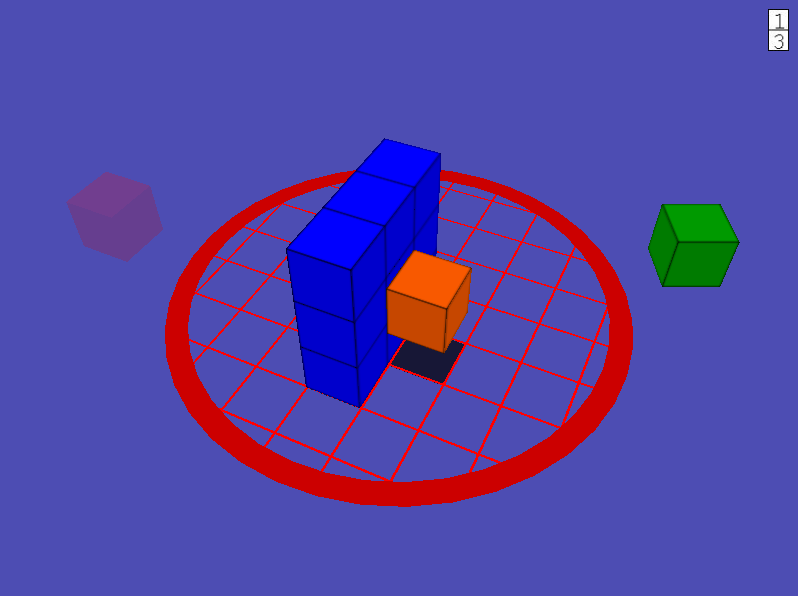
\includegraphics[width=0.47\textwidth ]{ghost_block}
\includegraphics[width=0.47\textwidth ]{Leap_hand}
\caption{\label{fig:ghostblock} \textit{On the left:} The ghost block (transparent-red block on the left) appeared when a block got stuck behind other blocks while dragging. 
In this case the user was dragging a building block from right to left, but the dragged block got stuck behind a wall of other building blocks. \textit{On the right:} The Leap 
Motion hand (transparent-green box for the palm, spheres for the finger-tops) was a visualization for when the Leap Motion device was able to detect one or more hands and the 
associated fingertips of a user. Additionally it indicated the  position of the hand palm and fingertips relative to the task environment coordinates. 
}
\end{figure}

\paragraph{Ghost block}
The ghost block was a special transparent-red block that had the same size as a normal building block. It only appeared when a building block was dragged but got stuck behind 
other blocks. Such a situation is depicted in Figure~\ref{fig:ghostblock} on the left. The ghost block helped the user to realize that an illegal dragging operation was being 
performed and what the current 3D location of the dragged building block would be if it would not have been stuck.


\paragraph{Leap Motion hand}
The Leap Motion hand visualizes the hand of the user when detected by the Leap Motion device and can be seen in Figure~\ref{fig:ghostblock} on the right. The Leap Motion 
hand was only visible to users interacting with the Leap Motion interface and helped to relate the relative position of the hands detected by the Leap Motion device to the 
coordinates of the task environment. Detected hand palms were represented as flat transparent-green boxes, where the position and orientation were determined by the position 
and orientation of the users hand palm relative to the Leap Motion device. Fingertips were represented with small transparent-green spheres and had positions relative to the
 fingertips of the user. Each individual fingertip and each hand palm was only shown when it was visible to the Leap Motion device and hidden otherwise.

\paragraph{Floor}
The floor was merely a purple-blue plane that indicates the lower limit to put the building blocks. It also served as a surface to project shadows from the building blocks on.

\paragraph{Horizon}
A small strip of horizon was made visible to help the user understand the orientation when tilting the camera up and down by changing the angle. The current color of the 
horizon was dark-gray.

\subsubsection{Color and lighting settings}

All the previously described components had one or more color states associated with them, depending on the state of the respective component and are listed in 
Table~\ref{tab:colors}. Each  color state consist out of a red (r), green (g), blue (b) and an alpha (a) component contributing to the color intensity and could 
optionally have a thin black border (outline) at the edges of the objects. Also all visual components, except the horizon, were influenced by two types of virtual lighting: 
\begin{enumerate}
	\item{\textbf{Ambient lighting:}} All color intensities were multiplied by $0.8$ on default.
	\item{\textbf{Parallel directional light:}} All the color intensities of non-transparent object surfaces perpendicular to the y-axis were restored to their original 
	color values.
\end{enumerate}


\begin{table}[H]
\centering
\begin{tabular}{|c|c|c|c|c|c|c|c|}
\hline
\textbf{object} & \textbf{state} & \textbf{r} & \textbf{g} & \textbf{b} & \textbf{a} & \textbf{outline} & \textbf{common name}\\ \hline\hline
Building block & resting & 0 & 0 & 255 & 255 & x & blue \\ 
 & dragged & 255 & 191 & 0 & 255 & x & orange \\ 
 & pointed & 138 & 149 & 255 & 255 & x & light-blue \\ \hline 
Creation block & resting & 0 & 178 & 0 & 255 & x & dark-green \\ 
 & pointed & 158 & 255 & 149 & 255 & x & light-green\\ \hline 
Ghost block & - & 255 & 0 & 0 & 51 & & transparent-red \\ \hline
Leap Motion hand & - & 0 & 255 & 0 & 77 & & transparent-green  \\ \hline 
Grid & resting & 255 & 0 & 0 & 255 & & red \\ 
 & rotating & 255 & 191 & 0 & 255 & & orange \\ \hline 
Floor & - & 77 & 77 & 179 & 255 & & purple/blue \\ \hline 
Horizon & - & 51 & 51 & 51 & 255 & & dark-gray \\ \hline 
\end{tabular}
\caption{\label{tab:colors} Color states of the objects within the task environment.}
\end{table}

\noindent The first reason for the different colors was that a user should be able to clearly differentiate between the components and their states within the environment. 
The outlines were added to the blocks blocks to enable the user to clearly distinguish between building blocks while they were immediately next to each other. Also, pilot
 tests without the `pointed' states for the creation block and the building blocks showed that some users struggled with identifying whether they were at the right position 
 with the Leap Motion hand to properly select and pickup blocks, thus the `pointed' states were included to make this more evident. 


\subsection{Control interfaces}\label{sec:interface}

The control interfaces define the actual control strategy, i.e. they describe the mapping from the input of a peripheral device towards the actual manipulations within the task environment. This section starts with a brief explanation of the two major sets of manipulations with the task environment and then discusses how these were implemented through control interfaces for the LEAP Motion and the mouse and keyboard. 

The major two sets of manipulations with the environment were:
\begin{enumerate}
	\item{\textbf{Building block manipulations:}} creating new blocks, dragging blocks, picking up blocks, dropping blocks and removing blocks.
	\item{\textbf{View manipulations:}} rotating the circular grid, lowering and raising the camera.
\end{enumerate}

\subsubsection{Keyboard and Mouse}

\paragraph{Building block manipulations}
In the keyboard and mouse interface, moving the block was solitary done with the mouse. To pick up a block the mouse button had to be clicked and held. As soon as the 
button was released, the block was also released. To move the block the mouse could be moved. However, to avoid flattening the environment to a 2D environment the movement 
of the mouse only determines the position in the 2D grid shown. To get the block higher, the scroll wheel of the mouse was used. The reason for doing this, is to make the 
comparison with the Leap Motion interface more fair. Because in the Leap Motion interface, there are also three dimensions in which the hand has to move.


\paragraph{View manipulations}
The view manipulations on the other hand were solitary done with the keyboard. In order to rotate the grid the left and right keys could be pressed respectively rotating the
 grid to the left or to the right at a constant pace. The up and down keys needed to be pressed in order to lift the camera up and down with a constant speed respectively.  
\subsubsection{Leap Motion}

\paragraph{Building block manipulation}
It was tried to keep the Leap M gesture as close to real life movements as possible. Therefore, the grabbing gesture had to be performed by closing a hand when it was 
shown above a block. The block was then shown inside the hand. While the hand remained closed the block would stay in the hand and move along with it. When the hand was opened 
the block would fall down at the position the hand was at that moment.

To indicate a grabbing gesture the function \texttt{Hand.scaleFactor(Frame sinceFrame)} from the Leap Motion SDK is used. This function looks at the scaling of the hand with 
all the fingers. When clenching the fist, the fingers get closer to the hand and therefore the scaling gets smaller, indicated by values $<1.0$. So for every frame, the program 
looks at the previous frame and finds a value of the scaling. When this value is lower than a certain threshold (in our case $<0.978$) it is saved. When the scaling gets lower 
for at least four frames, the system recognizes a grabbing gesture. When there are there are three or more frames in a row where the scaling is the same or bigger. The memory
 gets reset and the grabbing has to start over again.

After picking up it was easy to move the block, because the block would just follow the hand with which it was picked-up. Releasing was done in a similar manner as grabbing. 
When the scaling factor between the hand and the same hand in the previous frame was $>1.01$ for at least two frames the block got released. All thresholds were found with
 empirically.

An added feature to the Leap Motion interface was the fact that the hand should be near the block but not necessarily  on it to pick up the block. When detecting a grab gesture, 
the system would try to find a block within a certain parameter.

\paragraph{View manipulations}
The control of the circular grid through the Leap Motion is done by
swipe gestures. This choice was inspired by the numerous available
interaction patterns where swipe gestures are used to navigate through
some kind of interface. Also, a full hand swipe in a horizontal orientated
direction is similar to the movement one makes when spinning a plate
such as the circular grid. 

For these reasons a set of swipe gestures were implemented to rotate
the circular grid in both a horizontal and vertical direction (adjust
the angle at which the interface shows the grid). These gestures are
called the rotate gestures and are divided into two groups; swipe
gestures that move in a horizontal direction and those that move in
a vertical direction. The decision boundary lies at a $45$ degree
angle from the horizontal axis, any gestures beyond that angle are
classified as a vertical rotate gesture.

The straightforward implementation of these gestures based on the
swipe data presented by the Leap Motion and the used SDK caused several
problems. The first being that the SDK returned every swipe it detected
but not in a reliable way; the tags showing if this continuous gesture
just started, continued or ended in the current frame did not correlate
with the actual swipe movement performed. Therefore a single fluent
swipe performed by the user could contain several different swipes
according to the SDK. Another problem was that when the user made
an unrestricted swipe in open space there was always a small movement
back to a central position specific to the user. The SDK and Leap
Motion detected this movement as a swipe as well while not intended
as a rotate gesture. 

To solve these two problems a robust way of filtering the swipes received
from the SDK had to be created. This was done by creating two small
user profiles (one for each rotate gesture category) based on all
previous perceived rotate gestures started with some initial values.
This profile contained the average coordinate on the z-axis and x-axis
for respectively the horizontal and vertical rotate gestures. Each
category also contained the average speed of these gestures and the
average time between the rotate gestures. Each average was calculated
in a moving average manner as well as its moving standard deviation.
With these two values, and a static predefined sensitivity value,
a range was constructed where the respective feature should lie in
between to be accepted. If all features of a certain swipe were accepted,
the swipe was classified as a rotate swipe and was performed. 

The initial values of these user profiles was based on extensive trials
of three expert users using the rotate gestures. Their combined user
profiles was taken as these initial values. The sensitivity values
where also based on these trials to find their most optimal values.

The rotation of the circular grid based on the rotate gestures is
done in a momentum-decay manner; the velocity of the rotate gestures
contributes to the current rotation momentum of the circular grid
while at each frame this momentum was decreased by a certain decay
factor. This implementation was inspired on the various applications
where swipe is used to scroll the interface but is not immediately
stopped when no swipe is detected and where several swipes in quick
succession cause an increase in scrolling speed. 

The decay value and rotate gesture contribution (scaled by a sensitivity
value) differed for the vertical and horizontal rotate gestures. The
vertical rotate gesture had a larger decay value and large swipe velocities
did not affected the momentum as much (low sensitivity values). This
was due to a desire of changing the angle of the circular grid in
a more precise manner, whereas the horizontal rotate gesture did not
had such a requirement.

The usage of these small user profiles and extensive testing of several
sensitivity values resulted in a robust implementation of the rotate
gestures that could adapt on the users own preferred way of swiping.
The addition of a momentum-decay rotation effect caused the circular
grid to move in a more natural and intuitive way compared to previous
experience the user could have with swipe based navigation.
